\chapter{SCI-HI Data Analysis}\label{Ch:Data}

\section{Preparing the Data}
Before the data can be analyzed for potential signals, it first has to go through an analysis pipeline to remove noise and make the datasets easier to handle. 

\begin{figure}[htb]
\begin{center}
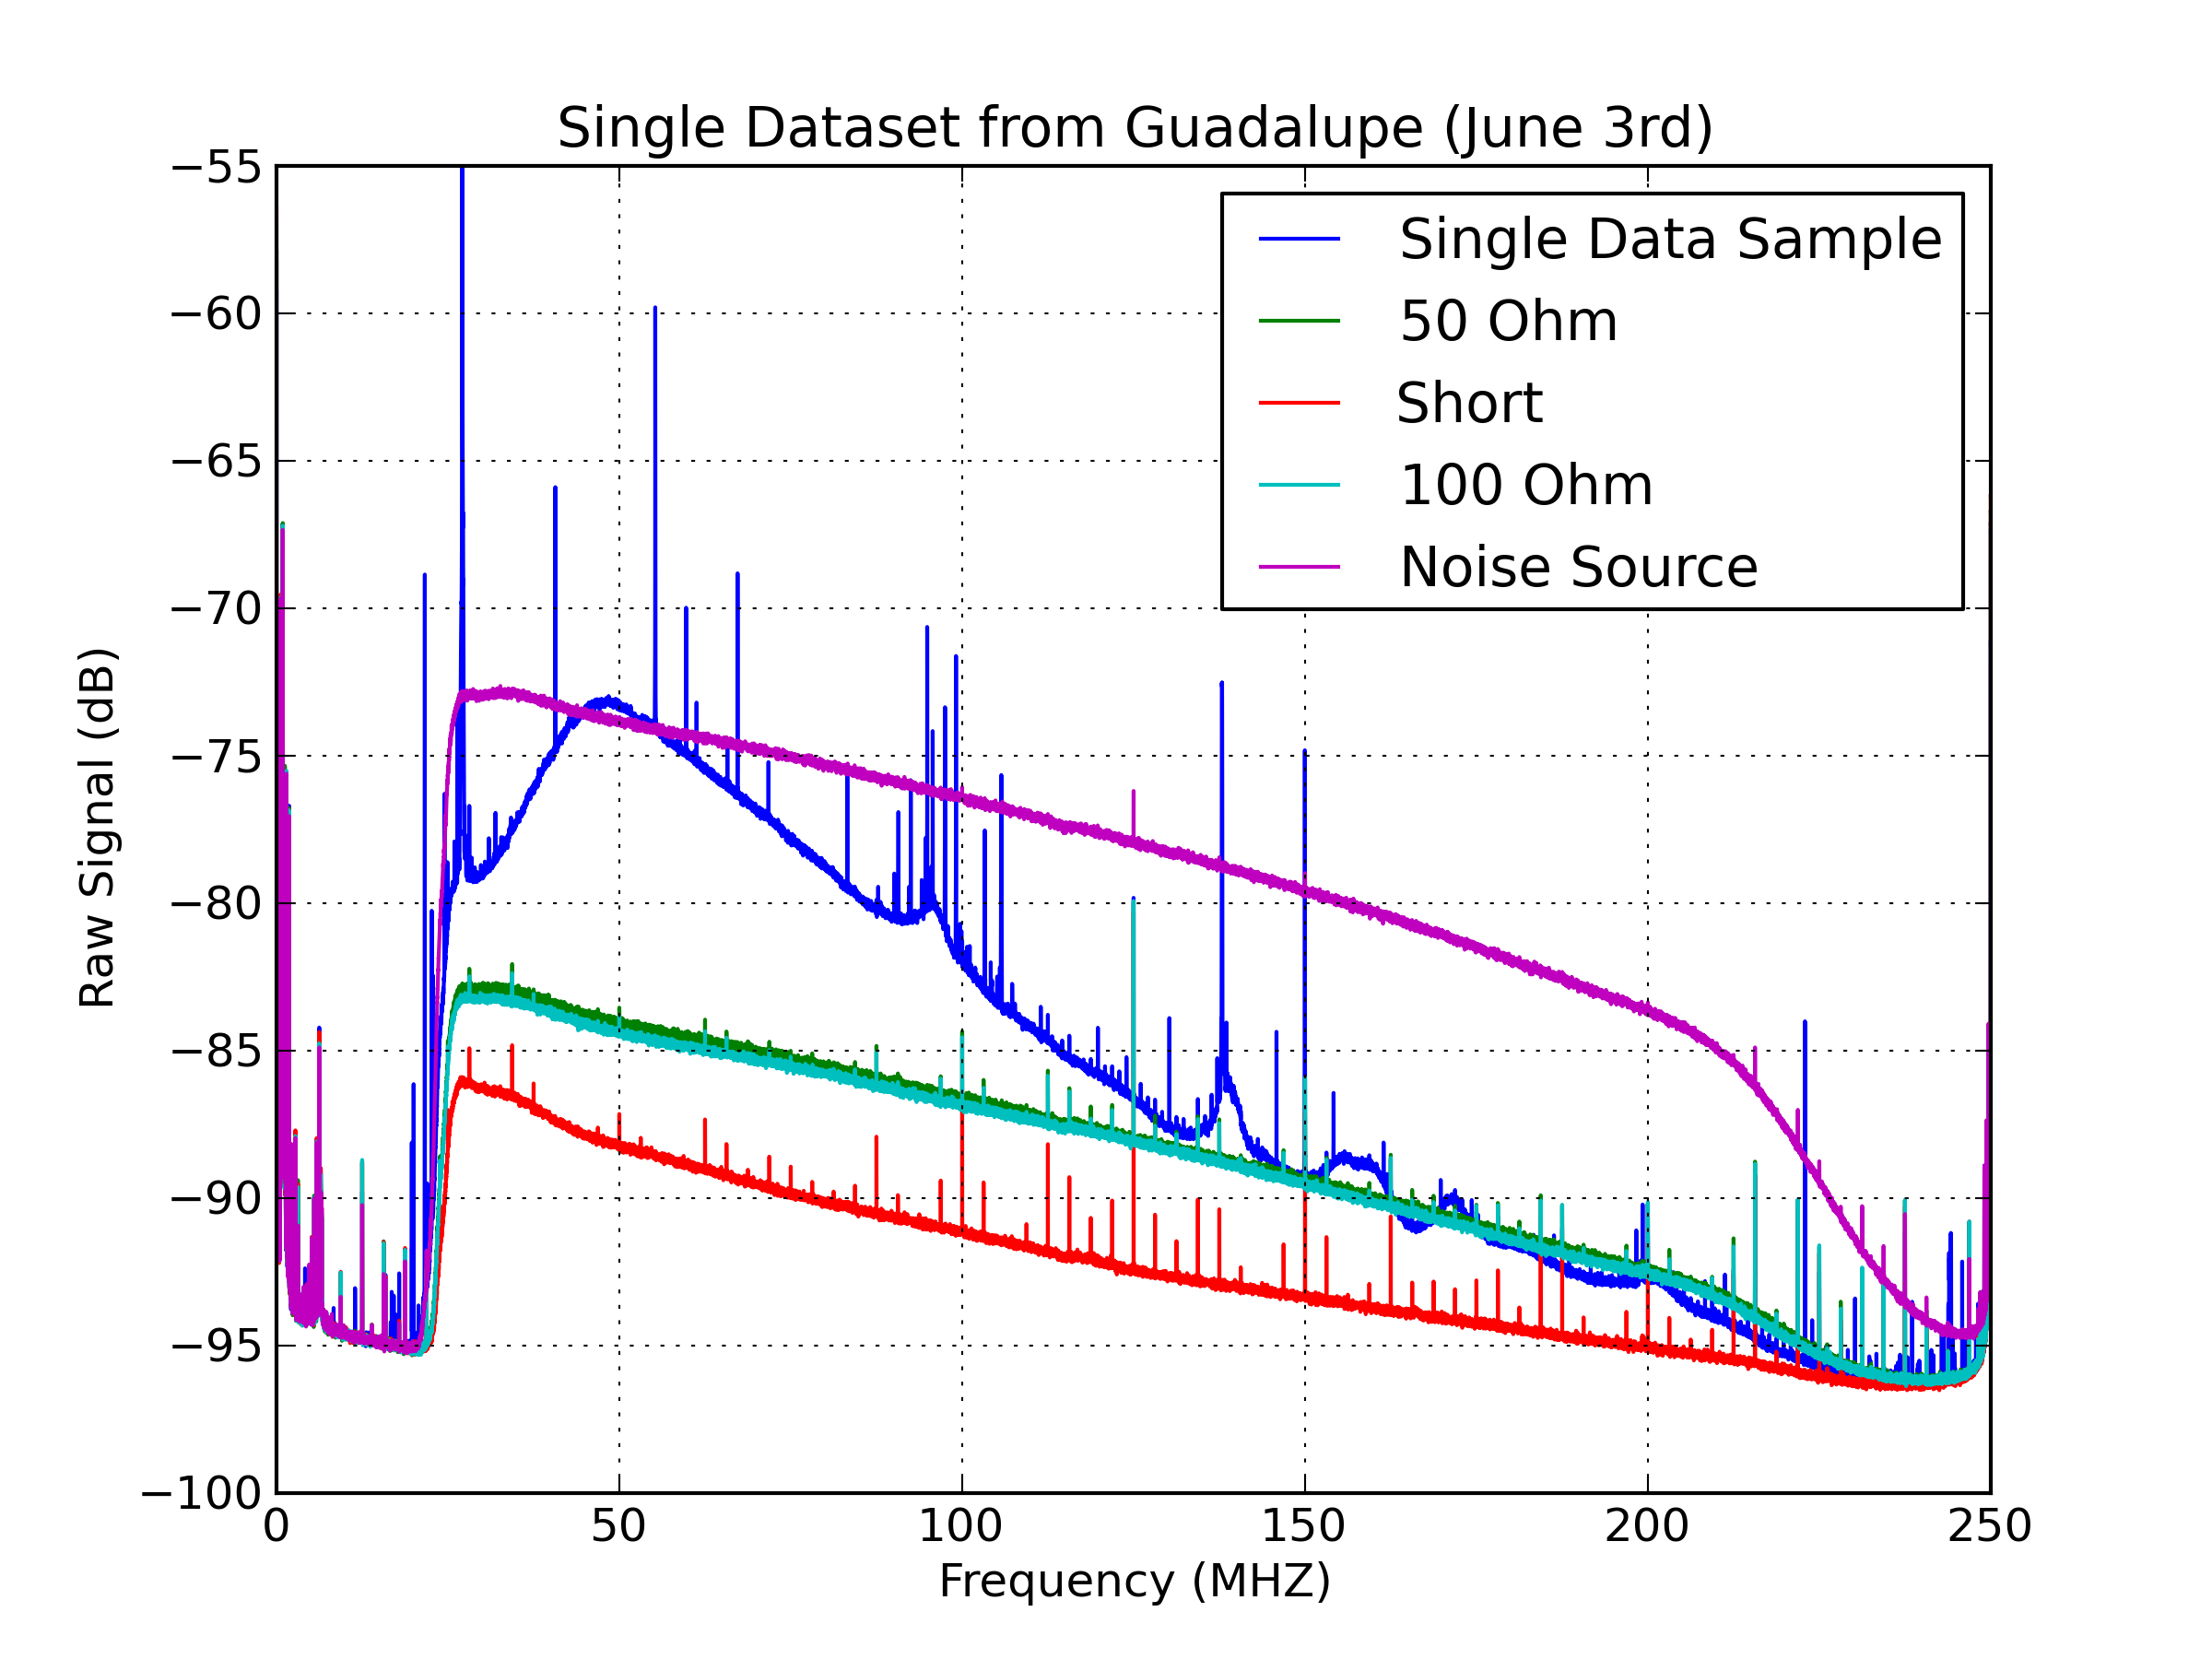
\includegraphics[width=0.9\linewidth]{Data_analysis/figures/single_raw_guad_june03.png}
\caption{Single dataset of the entire frequency spectrum of raw data from the SCI-HI system. Also present are single datasets from the different calibration sources.}
\label{Fig:raw_data}
\end{center}
\end{figure}

\subsection{Integration and Sampling}
The frequency spectrum collected for each second of data is stored in a single file with a header containing some basic information like the timestamp, DC voltage level (when measuring with DC Power Supply), computer temperature, and switch position (antenna vs calibration sources). The spectrum has a bandwidth of 250 MHz, with a frequency resolution of $\sim 7.63$ kHz (or 32769 samples). The data is in units of power (dB) as set by the data processing software. \textcolor{red}{I know there's something that Jose does to set these units but I'm not sure exactly what it is.} 

An example of the data collected by the system is shown in Figure \ref{Fig:raw_data}. Also included is a single sample of data from each of the calibration sources (Short, 50 $\Omega$, 100 $\Omega$, and Noise Source). The sharp signal cutoffs at 30 MHz and 200 MHz are from the high and low pass filters in the system.

\begin{figure}[htb]
\begin{center}
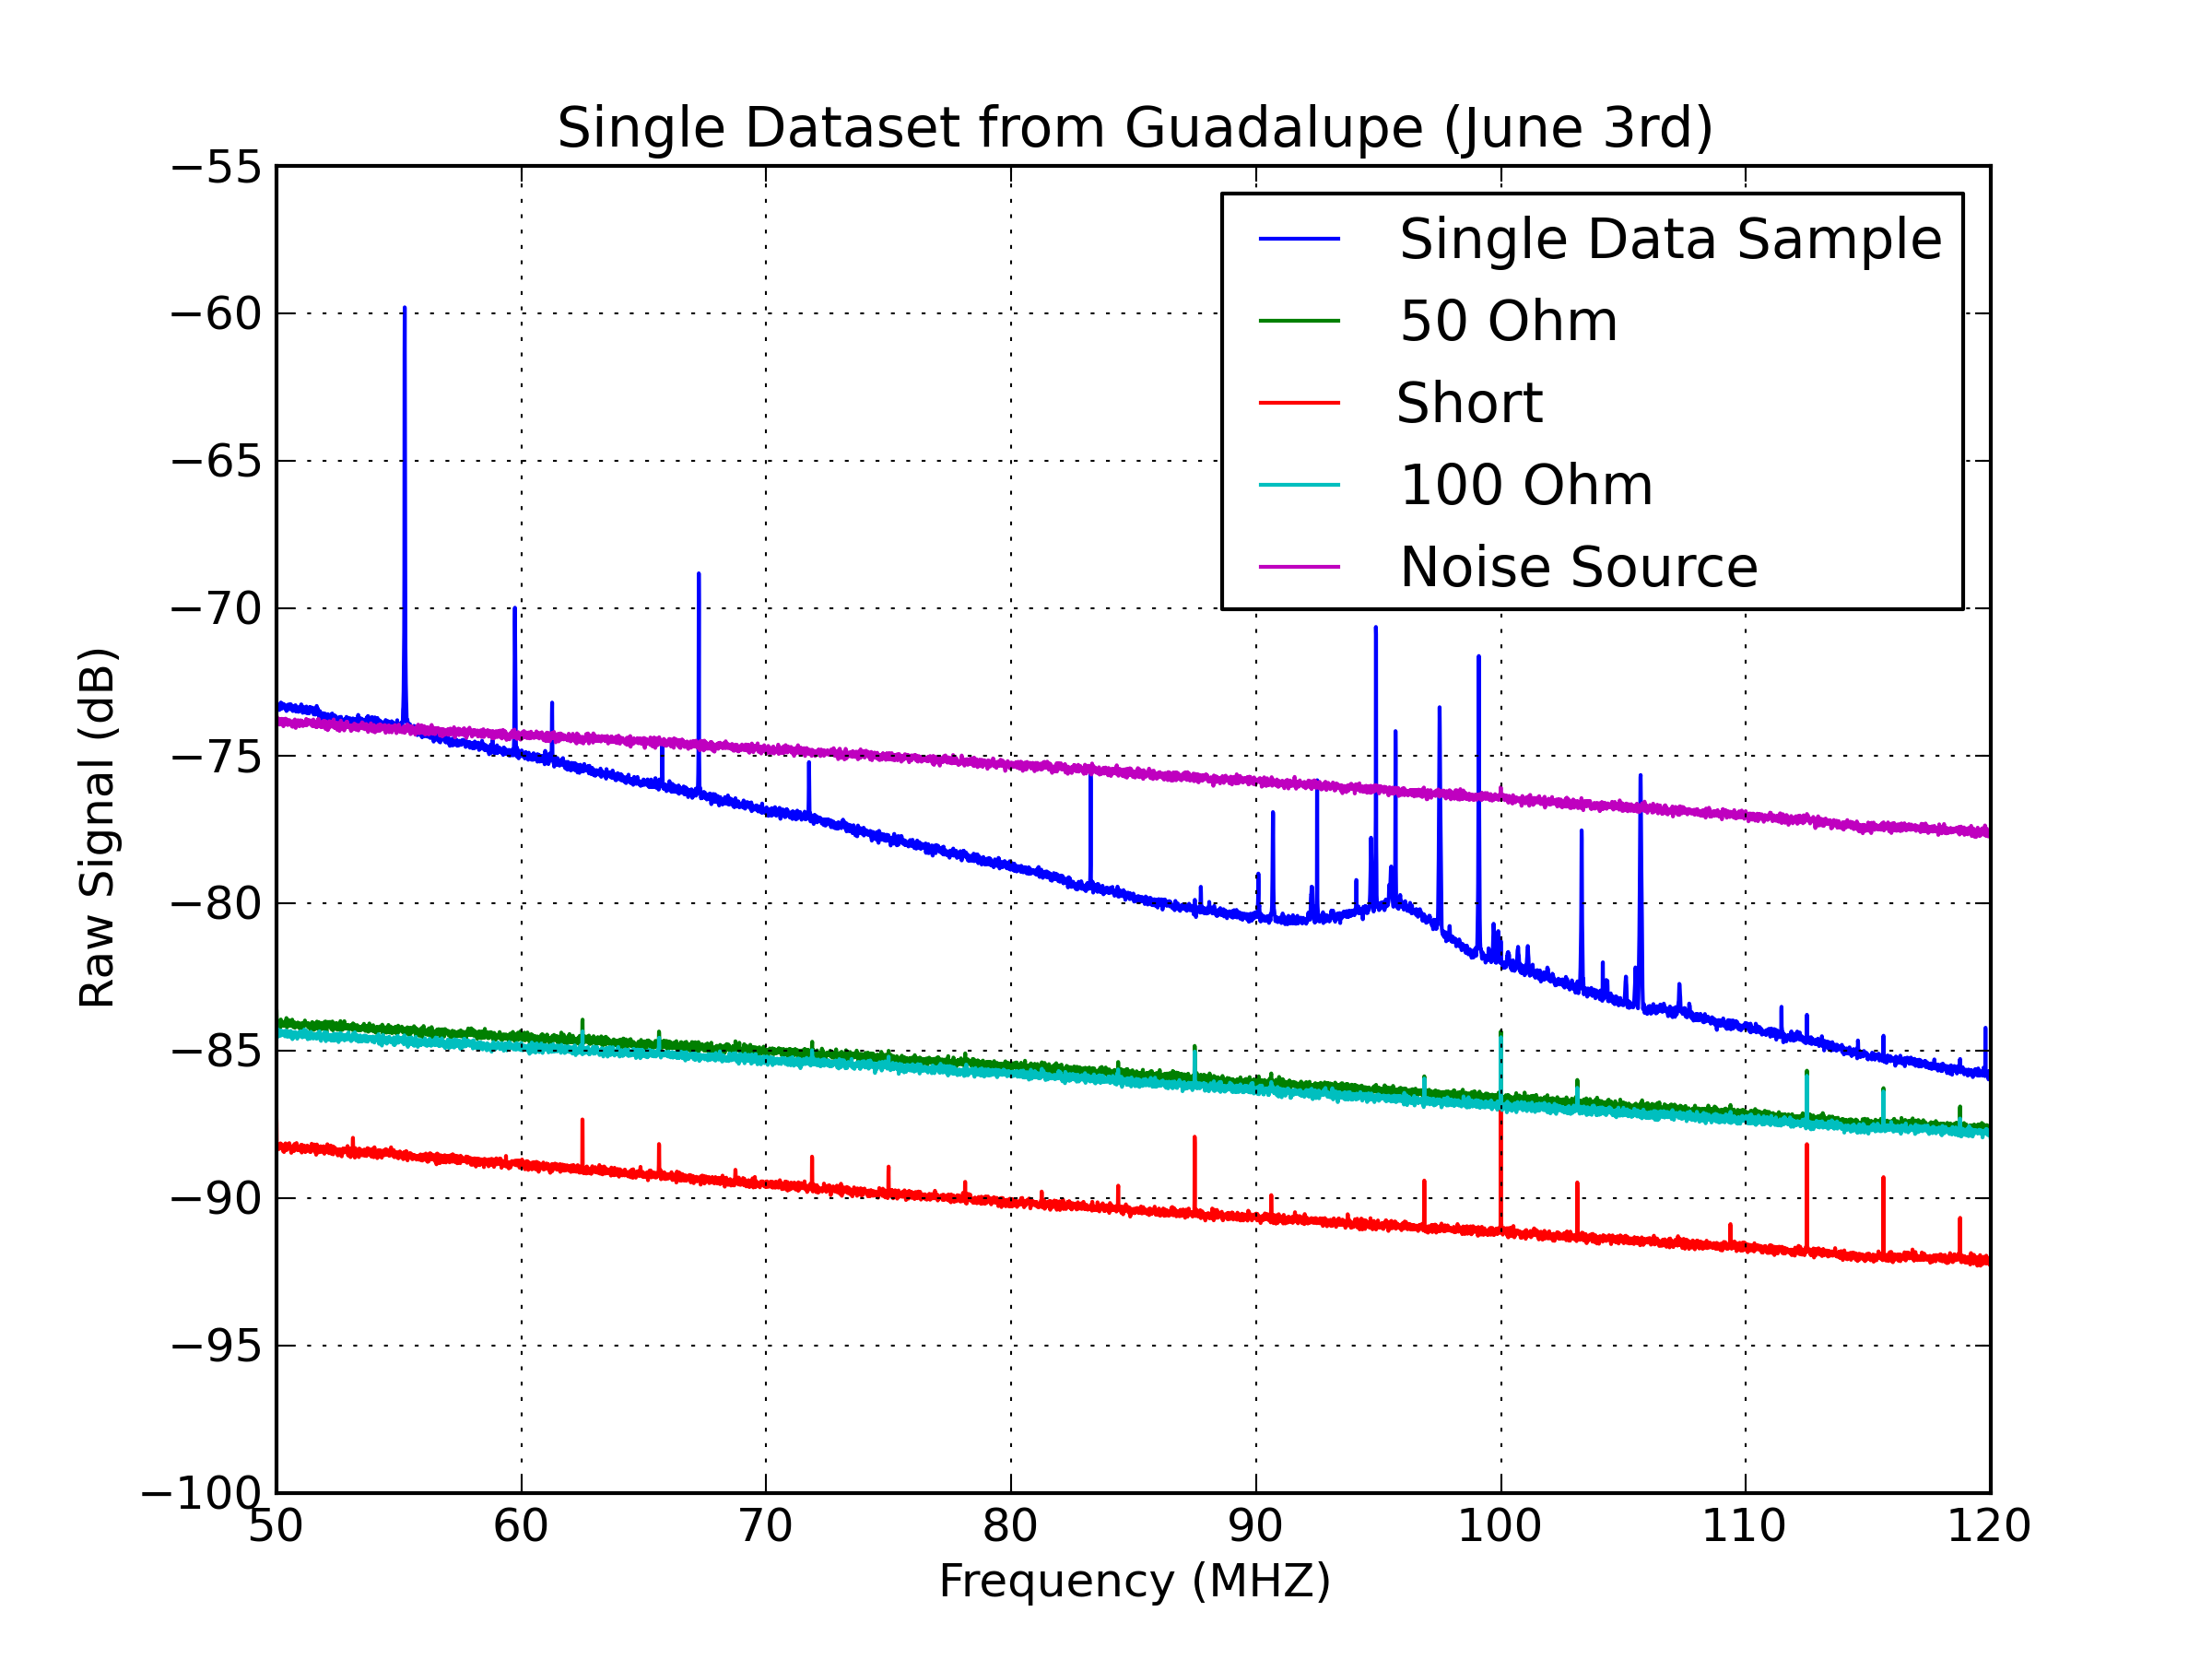
\includegraphics[width=0.9\linewidth]{Data_analysis/figures/single_raw_trunc_guad_june03.png}
\caption{Single dataset of a truncated spectrum of raw data from the SCI-HI system. Also present are single datasets from the different calibration sources.}
\label{Fig:raw_data_trunc}
\end{center}
\end{figure}

\subsection{Truncation}
Because the data we are interested in is a subset of the overall spectrum, one of the first things that we can do is to truncate frequency range of the data to make it smaller. For example, plotting the key frequency range for the SCI-HI data as collected in 2013 (50-120 MHz) helps us to pick out some of the things going on that are harder to see in the full spectrum (see Figure \ref{Fig:raw_data_trunc}). 

In the truncated dataset, it is easier to identify significant features in the data. For example, the nearly linear slope of the signal helps us confirm that the antenna is seeing the spectrum from the Milky Way Galaxy, while the excess of noise in the FM band and the bump in the middle of the FM band are evidence of RFI (both external and self-generated). 

\subsection{RFI Excision}
Another early stage of the pipeline is RFI excision (both in frequency and time). 

\subsubsection{RFI Frequency Flagger}
RFI excision in frequency is done using a flagger that does a threshold cut for each dataset. Because the data is expected to have a polynomial fit, the first step is to fit a two term polynomial to a small subset of the data (center frequency plus a its nearest neighbors). The subset of data is then divided by the polynomial and a mean and variance of the flattened data is calculated. If the data point at the center frequency is further from the mean than a set threshold, then that data point is flagged. 

The exact threshold and number of neighbors used to set the mean can be tweaked, but the typical values I used were a 3$\sigma$ threshold and 32 neighbors on either side. If a data point is flagged, it is masked out of the data and will not be included in the data in the future. 

\begin{figure}[htb]
\begin{center}
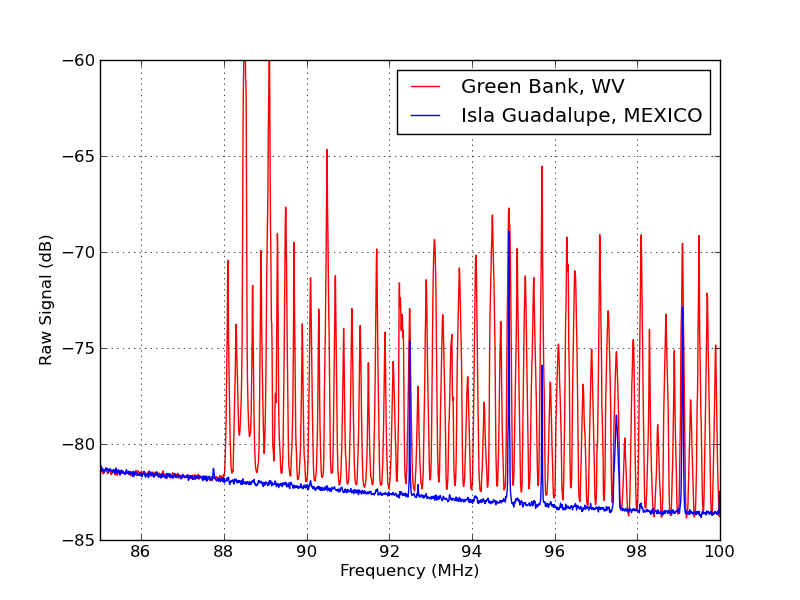
\includegraphics[width=0.9\linewidth]{Data_analysis/figures/FM_band_comp.png}
\caption{RFI comparison in the FM band between Isla Guadalupe and Green Bank, West Virginia. }
\label{Fig:FM_band}
\end{center}
\end{figure}

\subsubsection{RFI in the FM Band}
One of the frequency bands where RFI excision is particulary challenging is in the FM band (88-108 MHz). In this band, the variance of the signal can be quite large; making the RFI excision procedure less reliable. For many of our testing sites like Green Bank, WV the entire FM band is occupied with large RFI signals (as discussed in Chapter \ref{Ch:RFI}). This can be seen in Figure \ref{Fig:FM_band}, where the RFI signals are on average $\sim$10 dB above the floor. 

On the other hand, the FM band RFI signals from Isla Guadalupe are mostly $\leq$1 dB. These RFI signals are small enough to be missed by the RFI flagger and may be run through the rest of the pipeline stages. The few large spikes $\geq$5 dB above the floor will be removed by the RFI excision code. 

\subsubsection{Time-variable RFI}
While most of the RFI in the data is time indpendent and can be flagged out in each dataset indpendently, some of the RFI has a strong time-dependence. 

\paragraph{Time-variability of RFI due to Meteor Scatter}
Meteoroids are always passing through Earth's atmosphere. These meteoroids have a wide spectrum of sizes starting from $\leq$10 nm. As these meteoroids pass through the earth's atmosphere, some of their atoms are vaporized. Inelastic collisions between these atoms and air molecules in the atmosphere can lead to ionization \cite{meteor_review}. 

The result of this ionoization is a thickening of the Earth's ionosphere along the meteor trail, causing the ionosphere to become opaque to shorter wavelength photons along the trail. This opacity extends the range of signals such as FM radio to more distant locations than would normally be accessible.

In the SCI-HI data, this leads to a time-variable increase in the FM band RFI. For short time periods the strength of RFI signals from FM radio towers becomes larger. The duration of these signals is relatively small \textcolor{red}{(Add an estimate from our data based on the width of these events?)}, diminishing as free electrons diffuse away from the original meteor trail. 

\textcolor{red}{Add a plot here that shows a short time sample of RFI increase due to meteor scatter.}

\paragraph{Time-variability of RFI from Local Sources}
Another source of time-variable RFI is local noise from the surroundings. Our site at Isla Guadalupe was a few km from the local fishing village, which meant that occasionally RFI was picked up from the village when the diesel generator was powered on during the day. Additionally, the site was a few hundred meters from the road that led from the village to the rest of the island. When vehicles drove past the site (a few times each day), RFI from the vehicles such as broad band RF from spark plugs could be seen in the data. 

\subsubsection{Time-variable RFI Flagging}
In order to remove such time-variable RFI, I wrote a second RFI flagger identical to the frequency flagger, except that it works along the time axis. I typically used the same threshold and number of neighbors as the frequency flagger. 

\subsection{Rebinning}
Because the data is collected at a much higher resolution than is needed for the analysis, it needs to be rebinned to lower resolution. This can be done either in frequency or time. Compression is done after RFI flagging in order to keep a single $''$bad$''$ channel from affecting the overall signal. The mean of the unflagged data for a given bin scale becomes the new data point. In addition, a new data point is left as a flagged point if over half of the data used to make it were flagged. 

\section{Calibrating the Data}
After RFI removal and compression, the data is ready for calibration. 

\subsection{Calibration Datasets}

\subsubsection{Short Terminator}

\subsubsection{Load Terminators}

\subsubsection{Artificial Noise Source}

\subsubsection{On-site Impedence}

\subsection{Milky Way Galaxy (GSM) Modeling}

\subsection{Calibration Factor Calculation}

\subsubsection{Johnson Noise Calibration}

\subsubsection{Daily Variance with GSM Modelling}

\subsubsection{GSM and $\Delta$GSM Calibration}

\subsection{Calibration and Signal Loss}

\section{Removing the Foregrounds}

\subsection{Polynomial Fitting}

\subsection{Daily Residuals}

\subsection{Frequency Limitations}

